% Chapter 4

\chapter{Anisotropic Flow} % Main chapter title

%----------------------------------------------------------------------------------------

In the moments immediately after a collision event, the outwardly expanding behavior of the newly formed QGP can be studied to better understand the QCD processes that take place both during formation as well what happens as this QGP dissipates. Though it expands in all directions it is the expansion about the azimuth that best describes the behavior of this fluid. Often physicists like to describe the behavior of phenomena using a series expansion of orthogonal functions. Since the azimuthal angle runs from $0$ to $2 \pi$, this azimuthal expansion can be treated as a harmonic function which lends itself well to parameterization using a Fourier series. Recall that a Fourier series can approximate a function $f(x)$:

\begin{equation}
f(x) = \sum^{\infty}_{n=-\infty} A_{n} e^{i(2 \pi n x / L)}
\end{equation}
where
\begin{equation}
A_{n} = \frac{1}{L} \int^{L}_{0} f(x) e^{-i(2 \pi n x / L)} dx
\end{equation}

are said to be the Fourier \textbf{coefficients} or often, since they approximate harmonic functions, Fourier \textbf{harmonics}. It is a tautology that the exponential term can be written as the sum of a real cosine term and an imaginary sine term:

\begin{equation}
f(x) = \sum^{\infty}_{n=1} A_{n} cos (2 \pi n x / L) + i \sum^{\infty}_{n=1} B_{n} sin (2 \pi n x / L)
\end{equation}
where
\begin{equation}
A_{n} = \frac{1}{L} \int^{L}_{0} f(x) cos (2 \pi n x / L) dx 
\end{equation}
and
\begin{equation}
B_{n} = \frac{1}{L} \int^{L}_{0} f(x) sin (2 \pi n x / L) dx 
\end{equation}

Since we define $\phi=0$ to be along the waist of the ellipsoidal shaped QGP and not at the poles, odd function contributions (sine terms, $B_{n}$) to the Fourier series can all be ignored. 
Therefore if we wish to approximate the shape of the outgoing flow from the QGP we can define the rate of change of outgoing particle tracks vs transverse momentum and approximate it with a Fourier series. Flow anisotropy of the QGP can then be written as:

\begin{equation}
E \frac{d^{3}N}{dp^{3}} = \frac{1}{2 \pi} \frac{d^{2}N}{p_{T} dp_{T}dy}\Big( 1 + \sum^{\infty}_{n=1} 2 v_{n} \cos\big(n(\phi - \Psi_{r})\big) \Big),
\end{equation}

where:
\begin{equation}
v_{n} = \bigg \langle cos \Big( n [\phi - \Psi_{RP}]\Big) \bigg \rangle
\end{equation}

are the n-th order Fourier coefficients that describe the azimuthal shape of the QGP's outward expansion and $\phi$ is the azimuthal angle with respect to the reaction plane. Each n-th order coefficient scales the amount of expansion that behaves like $cos$ $nx$.

\begin{figure}[htbp!]
  \centering
    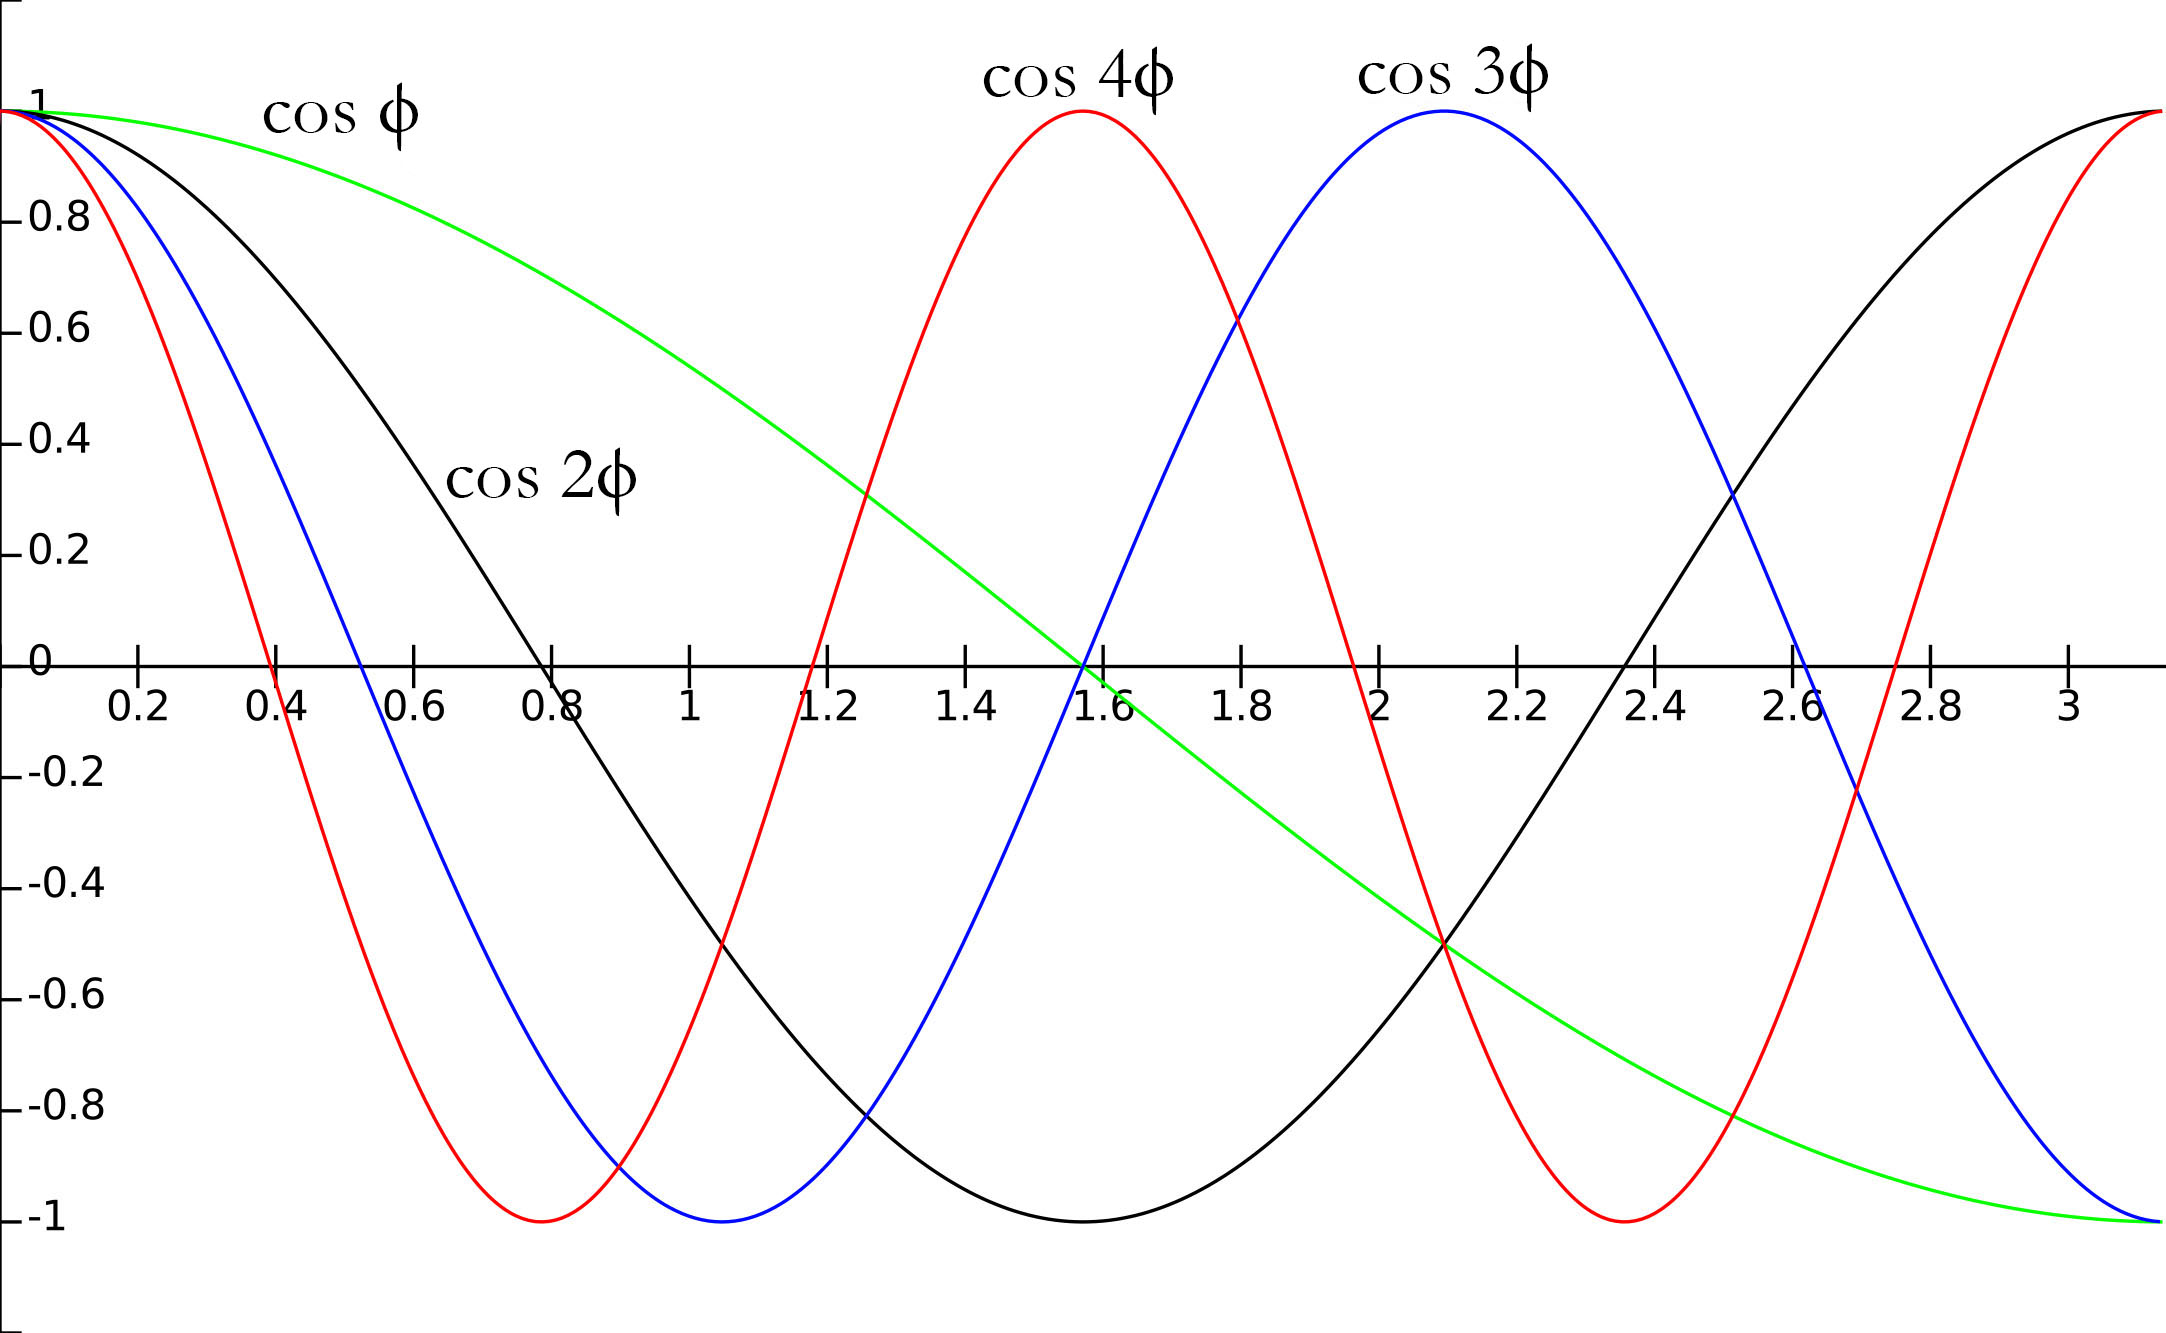
\includegraphics[width=0.8\textwidth]{Figures/fouriercosines.jpg}
    \rule{35em}{0.5pt}
  \caption[Plots of the first four harmonics of a cosine series]{Plots of the first four harmonics of a cosine series}
  \label{fig:fouriercosines}
\end{figure}

From studying the behavior of these various harmonics we can see that for $n=1$, $cos x$ is a maximum at $\phi=0$ and a minimum at $\phi = \pi$ which would correspond to a preferential flow in the $\phi=0$ direction. Therefore the $n=1$ flow coefficient is often called \textit{directed flow}. For the case of $n=2$ we see that again there is a maximum at $\phi=0$ and again at $\phi=\pi$ which corresponds to maximal flow at the waist of the ellipsoidal QGP. This expansion about the waist of the collision region results in an elliptical preferential flow, a term which is shortened to \textit{elliptic flow}. There are higher order harmonics which can describe various other phenomena of QGP flow which are beyond the scope of this analysis.

\pagebreak
\pagebreak
